%% ----------------------------------------------------------------
%% DesignImplementation.tex
%% ---------------------------------------------------------------- 
\chapter{Design \& Implementation} \label{Chapter:DesignImplementation}

To implement the neural network, a deep learning library is needed. Tensorflow with Keras API is chosen. 
\aref{Appendix:listing} shows the code to implement the LSTM model.

\begin{figure}[!htb]
    \centering
    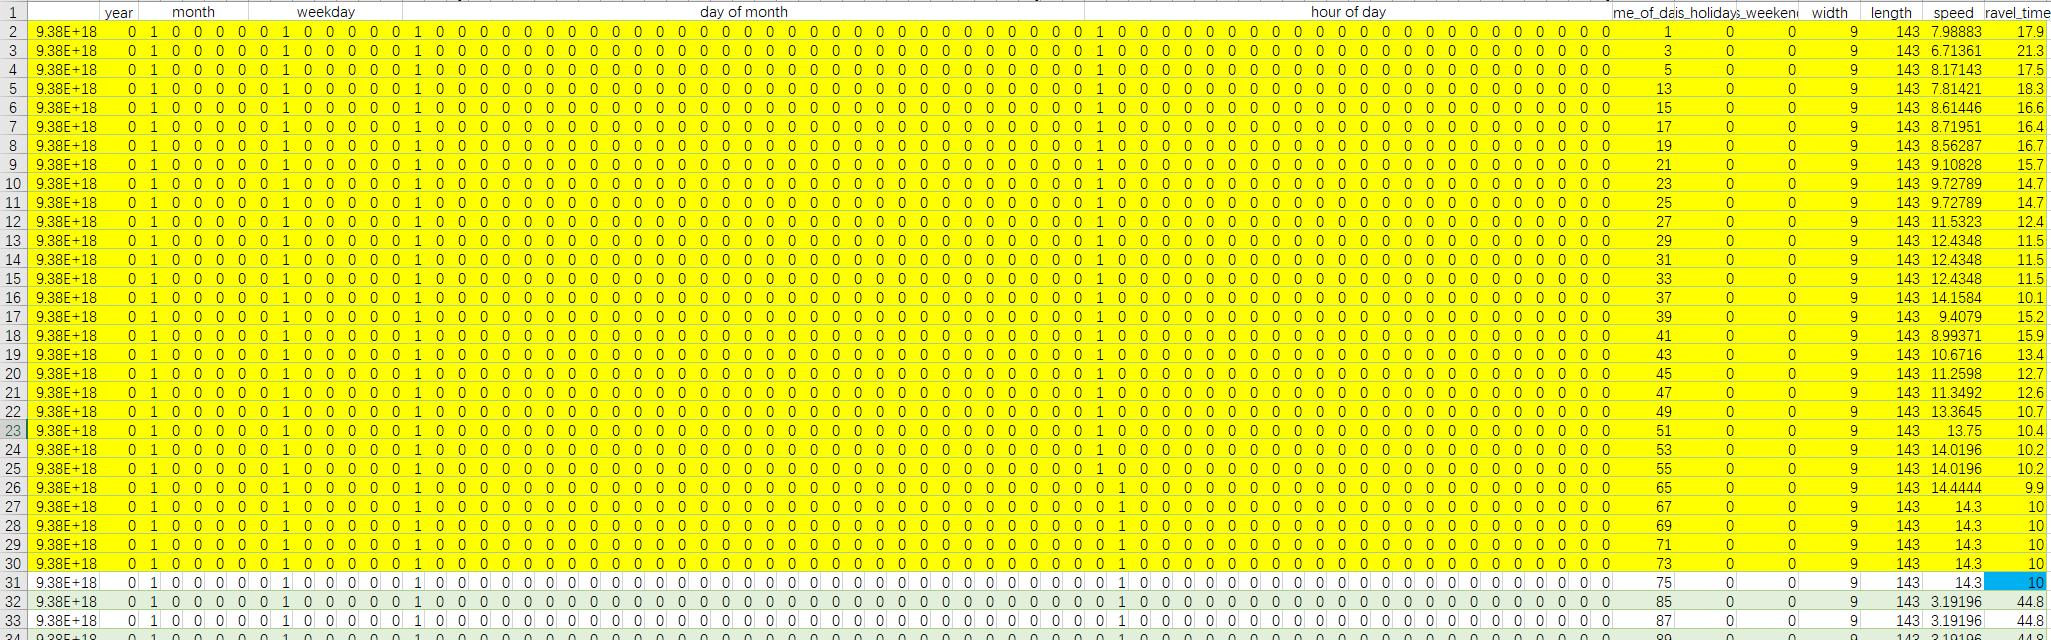
\includegraphics[width=14.5cm]{input shape}
    \caption{Yellow represents input structure; blue is the label as target}
    \label{Figure:input_shape}
\end{figure}

It is decided that to predict one sample, data from the previous 1 hour is used. For each sample, this gives an input shape of [30, 75], 30 being the previous 30 samples and 75 being the number of features.
Output shape is [1] since only the travel time will be predicted. \fref{Figure:input_shape} represents an example of one pair of inputs. 

The data have then been normalized, shuffled, and separated into training and validation sets, and it is ready to be fed into the model. The separation rate has been set to 0.9. 

\begin{figure}[!htb]
    \centering
    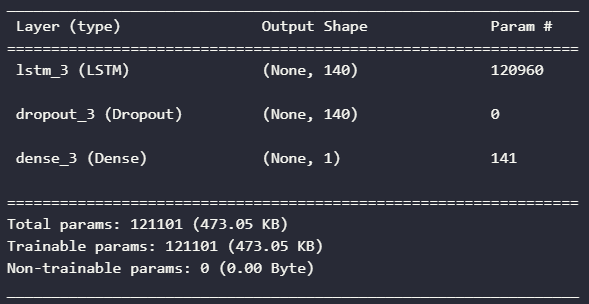
\includegraphics[width=12cm]{model_structure}
    \caption{A LSTM model constructed using Keras}
    \label{Figure:model_structure}
\end{figure}

A one-layer LSTM model is constructed, with a dropout layer of 0.2 and a dense layer, shown in \fref{Figure:model_structure}.

After 70 epochs, the model reaches its point of early stopping, with an MSE loss of $6.17\times 10^{-4}$. 

\begin{figure}[!htb]
    \centering
    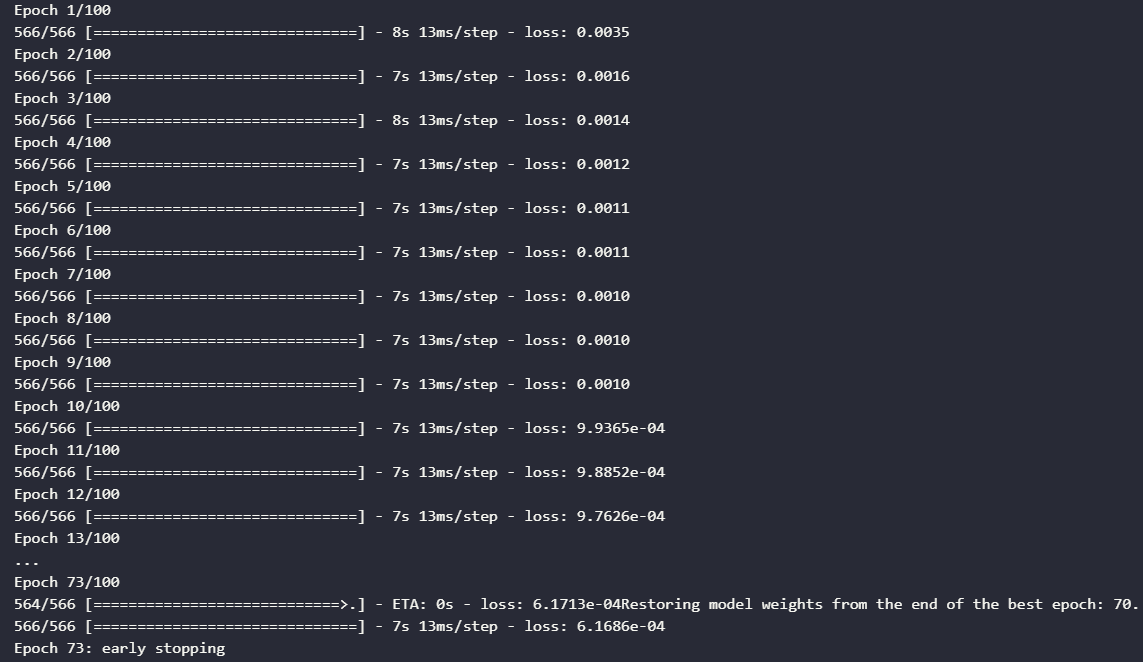
\includegraphics[width=12cm]{result1}
    \caption{Result}
    \label{Figure:result1}
\end{figure}

A plot of predicted value vs. target value is shown in \fref{Figure:result1_plot}. For this plot, the closer the points to the line $y = x$, the better the prediction is. 

\begin{figure}[!htb]
    \centering
    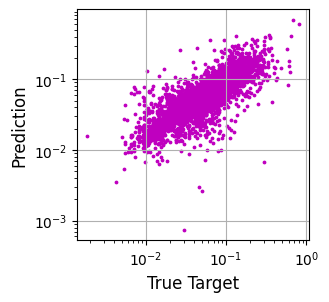
\includegraphics[width=8cm]{result validation}
    \caption{Predicted vs. target value}
    \label{Figure:result1_plot}
\end{figure}

